\documentclass{article}

% Packages
\usepackage[a4paper, total={210mm, 297mm}, includehead, includefoot,margin=2.5cm]{geometry}
\usepackage[english]{babel}
\usepackage{comment}
\usepackage{xcolor}
\usepackage{amsmath, amsfonts, amssymb}
\usepackage{float}
\usepackage{graphicx}
\usepackage{fancyhdr}
\usepackage{lastpage}
\usepackage{hyperref}
\usepackage{pagecolor}
\usepackage{mdframed}
\usepackage{lipsum}
\usepackage{url}
\usepackage{parskip}
\usepackage{mathtools}
\usepackage{centernot}
\usepackage{tcolorbox}


\usepackage{tikz}
\usetikzlibrary{arrows,decorations.markings}



% Settings
\hypersetup{colorlinks=true,linkcolor=black,filecolor=magenta,urlcolor=cyan}
\urlstyle{same}

\newcommand*{\QEDA}{\hfill\ensuremath{\blacksquare}}
\newcounter{pic}[page]
\newcounter{fig}[page]
\numberwithin{equation}{section}

\newmdtheoremenv[
	linecolor=IdealColour,
	leftmargin=60,
	rightmargin=40,
	outerlinecolor=IdealColour,
	outerlinewidth=2,
	roundcorner=60pt,
	backgroundcolor=white,
	innertopmargin=10pt,
]{example}{Example}[section]

\newmdtheoremenv[
	linecolor=IdealColour,
	outerlinecolor=IdealColour,
	outerlinewidth=2,
	roundcorner=60pt,
	backgroundcolor=LightGray,
	innertopmargin=10pt,
]{principle}{Principle}[section]

% Colours
\usepackage{xcolor}
\definecolor{HeadColour}{HTML}{376092}
\definecolor{IdealColour}{HTML}{ff6e6e}
\definecolor{LightGray}{gray}{0.9}
\renewcommand{\footrulewidth}{0.4pt}
\renewcommand{\baselinestretch}{1.5}

\pagestyle{fancy}
\fancyhead{}
\fancyfoot{}
\fancyhead[L]{\textbf{\textsc{IDEal}.}}
\fancyhead[R]{\today}
\fancyfoot[R]{Page \thepage \hspace{1pt} of \pageref*{LastPage}}

% Custom Commands
\newcommand{\ft}[1]{\mathcal{F}\{#1\}}
\newcommand{\Laplace}[1]{\ensuremath{\mathcal{L}{\left[#1\right]}}}
\newcommand{\InvLap}[1]{\ensuremath{\mathcal{L}^{-1}{\left[#1\right]}}}
\newcounter{NumberInTable}
\newcommand{\LTNUM}{\stepcounter{NumberInTable}{(\theNumberInTable)}}

\newcommand{\ideal}{\textsc{IDEal }}
\newcommand{\braket}[1]{\langle #1 \rangle}
\newcommand{\objectas}[2]{$\braket{#1 \ \text{as} \ #2}$}

\newcommand{\quickexample}[1]{
\begin{tcolorbox}
	\textbf{Example.} #1
\end{tcolorbox}
}

% Title
\date{\today}

\begin{document}

	\pagecolor{IdealColour}

	\begin{titlepage}
	\begin{center}
		\color{white}
		\vfill
		\line(1,0){400}\\[1mm]
			\huge{\textbf{IDEal: A Legal Development Environment}}\\
			\Large{\textbf{Australian Submission}}\\
			2020 \\
		\line(1,0){400}\\[3mm]
		\vfill
		\large{Mamta Thaker | Joanna Chen | Mirhady Dorodjatun | Joshua Fourie}
	\end{center}
	\end{titlepage}

	\pagecolor{white}

	\tableofcontents
	\thispagestyle{empty}
	\clearpage

\part{Business}

% TODO

%%%%%%%%%%%%%%%%%%%%%%%%%%%%%%% TECHNICAL PART %%%%%%%%%%%%%%%%%%%%%%%%%%%%%%%%%%%%

\pagebreak
\part{Technical}

A legal matter processed in \ideal traverses four states:
\begin{itemize}
	\item \textit{Generation} ($\mathcal{G}$). 
	\item \textit{Representation} ($\mathcal{R}$).
	\item \textit{Transformation} ($\mathcal{T}$). 
	\item \textit{Presentation} ($\mathcal{P}$).
\end{itemize}
	
We can understand \ideal as a system of \textit{plug-ins} which either generate, or commonly access and transform a unified representation of a legal matter into derivative states. Consequently, the system is a series of machines mapping $[ \ \alpha_i \in \mathcal{G} \ ] \rightarrow \mathcal{R}$, or $\mathcal{R} \rightarrow [ \ \mathbf{\alpha}_i \in \mathcal{T \cup P} \ ]$. We denote $\braket{\alpha_i}$ as a \textit{generator} state which can generate $\mathcal{R}$, and $\mathbf{\alpha}_i$ as a \textit{producible} state which be produced by some action on $\mathcal{R}$.
\begin{figure}[h]
\begin{center}
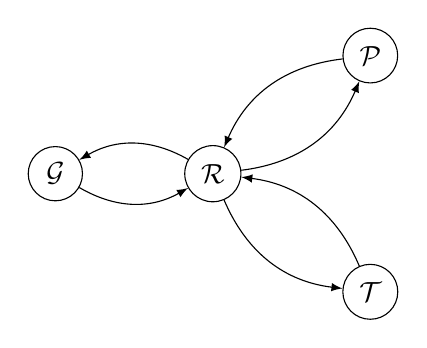
\begin{tikzpicture}
	\node[shape=circle, draw=black] (G) at (-2, 0) {$\mathcal{G}$};
	\node[shape=circle, draw=black] (R) at (0, 0) {$\mathcal{R}$};
	\node[shape=circle, draw=black] (T) at (2, -1.5) {$\mathcal{T}$};
	\node[shape=circle, draw=black] (P) at (2, 1.5) {$\mathcal{P}$};


	\path[->, >=latex] (G) edge[bend right] node {} (R);
	\path[->, >=latex] (R) edge[bend right] node {} (G);

	\path[->, >=latex] (R) edge[bend right] node {} (T);
	\path[->, >=latex] (T) edge[bend right] node {} (R);

	
	\path[->, >=latex] (R) edge[bend right] node {} (P);
	\path[->, >=latex] (P) edge[bend right] node {} (R);
	
\end{tikzpicture}
\end{center}
\caption{Visualising the interactions between the states.}
\end{figure}

In this section, we define $\mathcal{R}$, and provide an example of $(\mathcal{G} \rightarrow \mathcal{R})$ and $(\mathcal{R} \rightarrow \mathcal{P})$.


%%%%%%%%%%%% DEFINING THE REPRESENTATION %%%%%%%%%%%%%%%%%%%%%

\section{Defining the Representation}

Our goal is to define a mathematical structure for $\mathcal{R}$ which encodes legal information and maximises the number of producible states. Given that the representation is driven by the encoded legal information, we begin by discussing our generalisation of information relevant to a legal case.

%%%%%%%%%%%%%%%%%%%%% GENERALISING THE INFORMATION IN A LEGAL CASE %%%%%%%%%%%%%%%%%%%%%%%

\subsection{Generalising the Information in a Legal Case}

Generally, a lawyer functions as a mechanism for identifying the \textit{existence} or \textit{non-existence} of a legal relationship between \textit{objects}, as well as the extrapolation of any implications for a client. 

\paragraph{Facts, Nodes and the NodeState.} We describe a legal object as a \texttt{Node}, and define the \textit{factual} actions, attributes or character of the \texttt{Node} as the \texttt{NodeState}. The $\texttt{NodeState}_n$ is a set of $n$ \texttt{Fact} objects, $\texttt{NodeState}_n = \{ \ \texttt{Fact}_0, .., \ \texttt{Fact}_n \ \}$, which are generated and edited by an oracle, $\mathcal{F}$: % In the below, does a set of n always imply a nodestate of n?
\begin{align}
	\mathcal{F}: [ \ \{ \ \texttt{Fact}_0, .., \ \texttt{Fact}_n \ \} \rightarrow \texttt{NodeState}_n \ \ ] \\
	\mathcal{F}: [ \ (\texttt{Fact}, \ \texttt{NodeState}_n) \rightarrow \texttt{NodeState}_{n+1} \ ] \\
	\mathcal{F}: [ \ \texttt{NodeState}_n \rightarrow \texttt{NodeState}_{n-1} \ ]
\end{align}

\paragraph{Sources of Law.} A \texttt{SourceOfLaw} defines the conditions, attributes or characteristics which are required in order to generate the \texttt{Role} (\ref{section:role-object})  associated with a \texttt{NodeState}. Concretely, these are objects such as legislation or common law which have the inherent capacity to generate legal rights or obligations.

%%%%%%%%%%%%%%%%%%%%%%%%%%%%% ROLE %%%%%%%%%%%%%%%%%%%%%%%%%%%%%%%%%%%%%%%%%%%

\subsubsection{The Role Object} \label{section:role-object}

A \texttt{Role} defines the \textit{legal personality} of a \texttt{Node} by capturing the attributes, actions, or characterstics attributable under law. A \texttt{Node} can be subject to multiple \texttt{Role} objects of arbitrary complexity, provided they are distinct under (\ref{eq:role-equivalence}). The \texttt{Role} associated with a \texttt{Node} is generated by a pair \texttt{(NodeState, SourceOfLaw)} under the oracle function, $\mathcal{F}$, and is transformable under the \texttt{Consequence} of a \texttt{Link} (\ref{section:links-and-consequences}): 
\begin{align}	
	\mathcal{F} : [ \ \texttt{(NodeState, SourceOfLaw)} \rightarrow \texttt{Role} \ ] \\
	\texttt{Consequence} : [ \ \texttt{Role} \rightarrow \texttt{Role'} \ ]
\end{align}

\paragraph{Equivalence of Roles.} We define an equivalence relation on a pair $(\texttt{Role}_i, \ \texttt{Role}_j)$ by comparing their generating states, such that they are only pairwise distinct where the generative facts or law diverge:  
\begin{equation}\label{eq:role-equivalence}
[ \ \texttt{Role}_i = \texttt{Role}_j \ ] \iff [ \ (\texttt{NodeState}_i \iff \texttt{NodeState}_j) \land (\texttt{SourceOfLaw}_i \iff \texttt{SourceOfLaw}_j) \ ]
\end{equation}

\paragraph{Role Composition.} The \texttt{NodeState} of a \texttt{Node} can generate multiple \texttt{Role} objects \textit{iff} the (\texttt{NodeState, SourceOfLaw}) pair are distinct under (\ref{eq:role-equivalence}). A \texttt{Role} is \textit{reducible} where a subset of the generative pair (\texttt{NodeState, SourceOfLaw}) can produce another distinct \texttt{Role}:
\begin{align}
	N_n := \{ \ \texttt{Fact}_0, .., \ \texttt{Fact}_n \ \} \\
	[ \ \exists \ N' \subset N_n \ ] \implies [ \ \text{$N_n$ is reducible} \ ] 
\end{align}

A \texttt{Role} which is reducible is an \textit{extension} or \textit{composition} of another \texttt{Role}, and the \texttt{Role} objects which are extended are called the \textit{components of the extension}. The extended \texttt{Role} will automatically import any components of the extension objects into its own definition. We denote an extension using subset notation, such that the following indicates $\texttt{Role}_i$ is an extension of $\texttt{Role}_j$: $\texttt{Role}_j \subset \texttt{Role}_i$.

% Furthermore, whilst an automorphic \texttt{Link} over an irreducible \texttt{Role} is undefined behaviour, an extension can freely modify any components.

\paragraph{Role Substitution.} Given that an extension implies any components, a \texttt{Node} with multiple \texttt{Role} objects \textit{may} replace any \texttt{Role} with an extension:
\begin{align}
( \ \texttt{Role}_j \subset \texttt{Role}_i \ ) \implies ( \ \texttt{Role}_i \implies \texttt{Role}_j \ )
\end{align}

%%%%%%%%%%%%%%%%%%%%%%%%%%%%%%%%% LINKS AND CONSEQUENCES %%%%%%%%%%%%%%%%%%%%%%%%%%%%%%%%%%%%%%

\subsubsection{Links and Consequences}\label{section:links-and-consequences}

A \texttt{Link} is a directed, pairwise relationship between a source, $\texttt{Role}_i$, and a destination, $\texttt{Role}_j$, which has been generated by a \texttt{SourceOfLaw}. Given a pair $(\texttt{Role}_i, \texttt{Role}_j)$ and an associated $\texttt{Link}_{i \rightarrow j}$ drawn by the oracle, $\texttt{Role}_j$ is mapped into $\texttt{Role}_{j'}$ under some \texttt{Consequence}:
\begin{align}\label{eq:role-extension}
	\mathcal{F} : (\texttt{SourceOfLaw}, \ \texttt{Role}_i, \ \texttt{Role}_j) \rightarrow [ \ \texttt{Link}_{i \rightarrow j} \ ] \\
	\texttt{Link} \implies [ \ \texttt{Consequence} : \texttt{Role}_j \rightarrow \texttt{Role}_{j'} \ ]
\end{align}

\vspace{0.25cm}
\quickexample{
	Consider a contract, $\mathcal{C}$, between Alice, $\mathcal{A}$, and Bob, $\mathcal{B}$. We define $\mathcal{C}$ as a \texttt{SourceOfLaw}, and both $\mathcal{A}$ and $\mathcal{B}$ as parties to the contract. Consequently, there are two links: $\texttt{Link}_{\mathcal{A} \rightarrow \mathcal{C}}$ and $\texttt{Link}_{\mathcal{B} \rightarrow \mathcal{C}}$. The \texttt{Consequence} of any \texttt{Link} with $\mathcal{C}$ is that both $\mathcal{A}$ and $\mathcal{B}$ are bound by the contract, and whatever \texttt{Role} objects they possess are modified accordingly. Furthermore, the \texttt{Role} assigned to $\mathcal{A}$ and $\mathcal{B}$ as 'parties to the contract' is an extension of the 'legal person' role, and it is therefore implied under (\ref{eq:role-extension}).
}

\pagebreak
%%%%%%%%%%%%%%%%%%%%%%%%%%%%%%% DRAFT %%%%%%%%%%%%%%%%%%%%%%%%%%%%%

\paragraph{Compliance and Deviation.} A lawyer constructs a \texttt{Link(Consequence)} by analysing the \texttt{Role} of an object relative to a set of legal conditions. We define both compliance and deviation as:
\begin{equation}
[ \ \exists \ \texttt{Link(Existence, Consequence)} \ ] \land 
	\begin{cases}
		[ \ \texttt{Role} \implies \texttt{Link(..)} \ ], & \text{Compliance} \\
		[ \ \texttt{Role} \centernot\implies \texttt{Link(..)} \ ], & \text{Deviation}
	\end{cases}
\end{equation}

\vspace{0.25cm}
\quickexample{
	Continuing the previous example, we define compliance as Bob enforcing the terms of C against Alice, because Alice fulfils the relevant \texttt{Role}. Bob could not, however, enforce C against a third party, unless they also fulfilled a role which generated a \texttt{Link} to C.
}


% TODO: Actions progress Time?














\pagebreak
\section{Appendix A}

We discuss applications of the selected representation to cases.

\subsection{\textit{Belgrave Nominees v Barlin-Scott Airconditioning (Aust.)}}  

These are the objects involved in the \textit{Belgrave Nominees v Barlin-Scott Airconditioning (Aust.)} case:


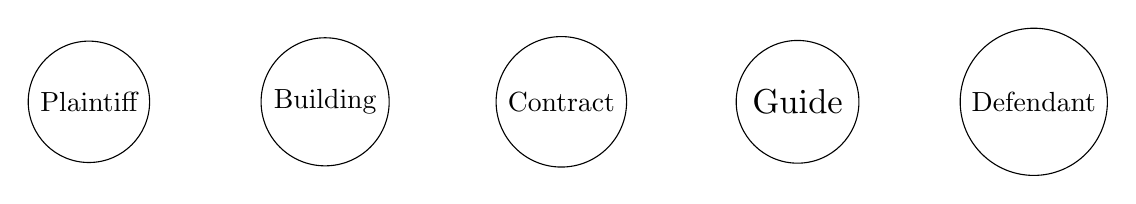
\begin{tikzpicture} 

	\node[shape=circle, draw=black] (Plaintiff) at (-10, 10) {Plaintiff};
	\node[shape=circle, draw=black] (Building) at (-7, 10) {Building};
	\node[shape=circle, draw=black] (Contract) at (-4, 10) {Contract};
	\node[shape=circle, draw=black, scale=1.25] (Guide) at (-1, 10) {Guide}; 
	\node[shape=circle, draw=black] (Defendant) at (2, 10) {Defendant};	

\end{tikzpicture}





















\pagebreak

\begin{example}{A Simple Relationship.}\label{david-builds-a-fence-on-patricias-land} ~\\
\textnormal{Consider the following: \textit{David builds a fence on Rosie's land without consent.}}

\vspace{0.25cm}

\begin{minipage}{0.45\textwidth}
\begin{tcolorbox}[left=1pt,right=2pt,top=1pt,bottom=0pt]
	From: \texttt{Rosie} \\
	To: \texttt{Land} \\
	Role: \texttt{SuperiorPossessor} \\
	Link: \texttt{(Yes, Modifier)}
\end{tcolorbox}
\end{minipage}
\hspace{0.75cm}
\begin{minipage}{0.45\textwidth}
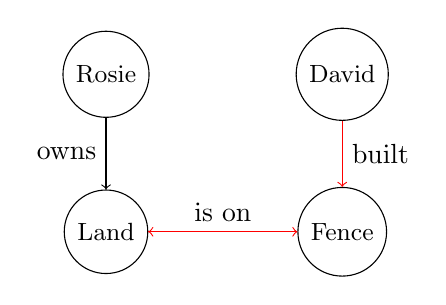
\begin{tikzpicture}
	\node[shape=circle, draw=black] (D) at (3, 2) {\small{David}};
	\node[shape=circle, draw=black] (F) at (3, 0) {\small{Fence}};	
	\node[shape=circle, draw=black] (L) at (0, 0) {\small{Land}};
	\node[shape=circle, draw=black] (P) at (0, 2) {\small{Rosie}};	
	
	\path[->, draw=red] (D) edge node[right] {built} (F);
	\path[->, draw=red] (F) edge node[right, above] {is on} (L);
	\path[->, draw=red] (L) edge node {} (F);
	\path[->] (P) edge node[left] {owns} (L);
\end{tikzpicture}
\end{minipage}


\textnormal{
We have implicitly assigned \textit{Rosie} the \texttt{Role} of superior possessor of the parcel of land. Consequently, we set $\texttt{Existence} := \texttt{Yes}$, and $\texttt{Consequence} := \texttt{Modifer}$.
}

\end{example}


\subsection{Mathematical Abstraction of a Legal Case}


We assume that a lawyer is responsible for (1) identifying the existence or non-existence of \textit{legal relationships}, and then (2) drawing conclusions about the implications of those relationships for a client. Their expertise is in determining the relevance of a particular relationship to a given case, where the relevance is guided by the severity or possibility of any consequence to a client.


\subsection{A Starting Point}

Suppose that there exists a universe of objects:
\begin{equation}
	\mathcal{U} := \{ \ \omega_i : \omega_i \ \text{is an object in the universe} \ \} \\
\end{equation}

Within the universe, an object may be in a directed, pairwise relationship with another object:
\begin{equation}
	\exists \ \omega_i : (\omega_i \ \sigma \ \omega_j) 
\end{equation}

We define any relationship as transitive:
\begin{equation}
	(\omega_i \rightarrow \omega_j \ \sigma \ \omega_k) \implies (\omega_i \ \sigma \ \omega_k)
\end{equation}

We also define each object discretely and uniquely: 
\begin{equation}
		[ \ (\omega_i \ \sigma \ \omega_j) = (\omega_k \ \sigma \ \omega_{\ell}) \ ] \implies [ \ (\omega_i \iff \omega_k) \land (\omega_j \iff \omega_{\ell}) \ ]
\end{equation}





























\paragraph{Equivalence.} 
We define an equivalence relation on any machine acting on a given representation:
\begin{equation}
[ \ M_i(\mathcal{R}) = \alpha_i \ ] \land [ \ \alpha_i = M_j(\mathcal{R}) \ ] \ \implies \ [ \ M_i \Leftrightarrow M_j \ ]
\end{equation}

However, for the pair $(\mathcal{R}_i, \mathcal{R}_j)$:
\begin{equation}
[ \ M_i(\mathcal{R}_i) = \alpha_i \ ] \land [ \ \alpha_i = M_j(\mathcal{R}_j) \ ] \centernot\implies [ \ M_i \Leftrightarrow M_j \ ] \lor [ \mathcal{R}_i \Leftrightarrow \mathcal{R}_j.
\end{equation}




\end{document}
